% This file was converted to LaTeX by Writer2LaTeX ver. 1.0.2
% see http://writer2latex.sourceforge.net for more info
\documentclass[a4paper]{article}
\usepackage[utf8]{inputenc}
\usepackage[T3,T1]{fontenc}
\usepackage[slovene,english,french]{babel}
\usepackage[noenc]{tipa}
\usepackage{tipx}
\usepackage[geometry,weather,misc,clock]{ifsym}
\usepackage{pifont}
\usepackage{eurosym}
\usepackage{amsmath}
\usepackage{wasysym}
\usepackage{amssymb,amsfonts,textcomp}
\usepackage{color}
\usepackage{array}
\usepackage{supertabular}
\usepackage{hhline}
\usepackage{hyperref}
\hypersetup{pdftex, colorlinks=true, linkcolor=black, citecolor=black, filecolor=black, urlcolor=black, pdftitle=OpenWIM, pdfauthor=Ivan, pdfsubject=, pdfkeywords=}
\usepackage[pdftex]{graphicx}
\usepackage[alf,utf8,recuo=8pt]{abntex2cite}


% Text styles
\newcommand\textstyletablecaptionCar[1]{\foreignlanguage{english}{\textbf{#1}}}
% Outline numbering
\setcounter{secnumdepth}{2}
\renewcommand\thesection{\arabic{section}}
\renewcommand\thesubsection{\arabic{section}.\arabic{subsection}}
\makeatletter
\newcommand\arraybslash{\let\\\@arraycr}
\makeatother
% List styles
\newcommand\liststyleWWNumvi{%
\renewcommand\theenumi{\arabic{enumi}}
\renewcommand\theenumii{\arabic{enumii}}
\renewcommand\theenumiii{\arabic{enumiii}}
\renewcommand\labelitemi{[F0B7?]}
\renewcommand\labelenumi{\theenumi.}
\renewcommand\labelenumii{\theenumii.}
\renewcommand\labelenumiii{\theenumiii.}
}
% Page layout (geometry)
\setlength\voffset{-1in}
\setlength\hoffset{-1in}
\setlength\topmargin{2.501cm}
\setlength\oddsidemargin{2.501cm}
\setlength\textheight{24.698002cm}
\setlength\textwidth{15.999001cm}
\setlength\footskip{0.0cm}
\setlength\headheight{0cm}
\setlength\headsep{0cm}
% Footnote rule
\setlength{\skip\footins}{0.119cm}
\renewcommand\footnoterule{\vspace*{-0.018cm}\setlength\leftskip{0pt}\setlength\rightskip{0pt plus 1fil}\noindent\textcolor{black}{\rule{0.25\columnwidth}{0.018cm}}\vspace*{0.101cm}}
% Pages styles
\makeatletter
\newcommand\ps@Standard{
  \renewcommand\@oddhead{}
  \renewcommand\@evenhead{}
  \renewcommand\@oddfoot{}
  \renewcommand\@evenfoot{}
  \renewcommand\thepage{\arabic{page}}
}
\makeatother
\pagestyle{Standard}
\setlength\tabcolsep{1mm}
\renewcommand\arraystretch{1.3}
% footnotes configuration
\makeatletter
\renewcommand\thefootnote{\arabic{footnote}}
\makeatother

%\bibliographystyle{plain}
\bibliographystyle{abntex2-alf}

\def\citeay#1{\citeauthor{#1} (\citeyear{#1})} % Super!!!!!

\title{Universidade Federal de Santa Catarina}
\author{Ivan Ogassavara}
\date{2016-02-14}
\begin{document}
\clearpage\setcounter{page}{1}\pagestyle{Standard}
{\centering\selectlanguage{english}\bfseries
OpenWIM - Open Science and Weigh-in-Motion Research
\par}

\footnote{
$\copyright$ 2016, GOLTSMAN, Helio and OGASSAVARA, Ivan. Licensed under the Creative Commons Attribution 4.0 license, http://creativecommons.org/licenses/by/4.0/
}

\bigskip

\begin{flushleft}
\tablehead{}
\begin{supertabular}{m{3.8749998cm}m{3.8760002cm}m{3.8760002cm}m{3.8749998cm}}
\selectlanguage{english} Technologist researcher graduated from the Faculty Eniac, specialized in Information Systems at the Graduate Center Eniac. Experience in algorithms for moving vehicle weight estimation. &


\includegraphics[width=2.619cm,height=3.307cm]{openwim-img/openwim-img1.png}
 &

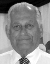
\includegraphics[width=2.619cm,height=3.307cm]{openwim-img/openwim-img2.jpg}
 &
\selectlanguage{english} Engineer researcher graduated from PUC-RJ, specialized in urban transportation planning by \ textit {Massachusetts Institute of Technology - MIT}. It was also one of the pioneers of the weighing area of heavy vehicles in Brazil, working since 1974 on this issue.\\
\multicolumn{2}{m{7.951cm}}{\centering
{\selectlanguage{english}\bfseries Ivan Ogassavara}\par

\centering {\selectlanguage{english} Universidade Federal de Santa Catarina}\par

\centering \selectlanguage{english} Brazil} &
\multicolumn{2}{m{7.951cm}}{\centering
{\selectlanguage{english}\bfseries Helio Goltsman}\par

\centering {\selectlanguage{english} Universidade Federal de Santa Catarina}\par

\centering \selectlanguage{english} Brazil}\\
\end{supertabular}
\end{flushleft}

\bigskip


\bigskip

{\selectlanguage{english}\bfseries
Abstract}

{\selectlanguage{english}

Abstract ...

}


\bigskip


{\selectlanguage{english}
\textstyletablecaptionCar{Keywords:} \ Heavy
Vehicles, Weigh-in-Motion, WIM, Open Science, Open Data, Reproducibility.}


\bigskip

{\selectlanguage{english}\bfseries
\foreignlanguage{portuguese}{Resumo}}

{\selectlanguage{english}
\foreignlanguage{portuguese}{
Resumo...
}}


\bigskip

{\selectlanguage{english}
\textstyletablecaptionCar{\foreignlanguage{portuguese}{Palavras-Chaves:}}\foreignlanguage{portuguese}{
Veículos Pesados, Pesagem em Movimento, WIM, Ciência Aberta, Dados Abertos, Reprodutibilidade}}

\section{Introduction}
{\selectlanguage{english}

Overweight heavy vehicles represent a problem related to accidents and pavement damage. The weight enforcement is very important to inhibit the overweight of these vehicles. One method that is being investigated in many parts of the world is weigh-in-motion (WIM), which has the advantage of reduced physical space required and operating with lower costs. Since the sensors can be installed on the road itself, the vehicles can be weigh without them having to slow down, hence, not delaying the road user’s journey.

Although there are many papers publicly available about weigh-in-motion, a little bit researchers publish their sources and data, which can allow a better reproduction of their experiments and results. In this context, the Open Science concept can help improve the WIM research through collaborative efforts and reproducible methods, using algorithms and data with open access.

The OpenWIM project was born upon this background as an open science initiative, to provide a WIM researchers a repository with initial structure that can then be converted into a framework for researchers to develop and test new methods and technologies.

The structure of this project was designed over some pillars:
\begin{itemize}
\item Standards;
\item Open Data;
\item Open Source;
\item Open Access.
\item Reproducibility;
\end{itemize}

The Standards pillar is based on a recompilation of standards found in the international literatures used in WIM projects. This can be a guideline to new researchers to structure their projects and can facilitate sharing data and algorithms. This standards can be about the file names, layout data structure, file format used in system integration, standard units, column name standard (in data files), algorithms style code, etc.

The Open Data pillar is based on a open repository where Weigh-in-Motion data is published. This data can be:

\begin{itemize}
\item raw data from weigh sensors;
\item raw data from inductive loop;
\item known information about the vehicle run (gross vehicle weight, speed, distance between axles, weight in each axle, vehicle category, temperature, etc.);
\item vehicle category patterns;
\item calibration data;
\item license plate images;
\item vehicle images;
\end{itemize}

The raw data from sensors and the weight information is very important to validate weigh and calibration methods. Raw data from inductive loop can help in methods like vehicle classification. The license plate images can help to test or improve methods that recognizes the license plate position and value.

The Open Source pillar is based on a repository for researchers publish his algorithms used in their research. This algorithms with a test dataset (open data) can help others in their research that allows more alternatives in their experiments. Other important key about this pillar is the informal peer-review because when other researchers can test some algorithms they can find some problem or exception or just can give some feedback.

The Open Access pillar is based on paper publishing on open repositories. This concept can allow a collaborative environment for researchers of all parts of the world to work and can increase paper citation.

The Reproducibility pillar is achieved through open access, open data and open source. To share code, explain and describe the methods, in a reproducible way, a \textit{notebook science} tool can be used. With that, the researchers can write texts, including texts with LaTeX format and algorithms; open data files; plot charts; display tables; show images; etc. Jupyter Notebooks, the most famous notebook science tool, can be used with some famous programming languages like Python, Julia, Octave, Bash, Scheme, etc.

This paper will shows the idea of the OpenWIM project and its potential benefits.

\begin{small}
\renewcommand{\bibname}{References}
\addcontentsline{toc}{section}{\bibname}
\bibliography{openwim}
\end{small}

\end{document}
